\documentclass[../main.tex]{subfiles}
\graphicspath{{../figures/}}

\begin{document}

\mychapter{绪\hskip\ccwd{}论}
\label{sec:ch1-preface}

\mysection{研究背景与意义}
\label{sec:ch1-1-research-background-and-significance}

深度学习领域正处在一个前所未有的关键节点。从 2012 年 AlexNet 在 ImageNet 竞赛中的突破性胜利开始\cite{imagenetclassificationdeep_krizhevsky_2012,imagenetlargescale_deng_2009},我们见证了人工智能技术的飞速发展,模型规模从百万级参数扩展到万亿级参数\cite{switchtransformersscaling_fedus_2021,gpt4technical_openai_2023},应用场景从简单的图像分类扩展到复杂的多模态生成任务\cite{highresolutionimage_rombach_2022}。然而,这种指数级的性能提升背后隐藏着一个日益严峻的核心矛盾:模型性能的持续增长与计算资源消耗的指数式攀升之间的不可调和性\cite{energypolicyconsiderations_strubell_2019,carbonfootprintmachine_patterson_2021}。这一矛盾不仅制约着深度学习技术的广泛应用,更对其可持续发展构成了根本性挑战。

\mysubsection{深度学习发展概述}\label{sec:ch1-1-1-deep-learning-overview}

自 2012 年 Hinton 等人凭借 AlexNet 在 ImageNet 大规模图像识别竞赛中取得突破以来,深度神经网络模型的性能不断攀升\cite{imagenetclassificationdeep_krizhevsky_2012}。AlexNet 的出现使得图像分类准确率相较于传统方法实现了质的飞跃:在当年的 ImageNet 竞赛中,AlexNet 将前一年的错误率从 26\% 大幅降低至 15\%,首次证明了大规模深层神经网络在复杂视觉任务上的巨大潜力\cite{imagenetclassificationdeep_krizhevsky_2012}。这一里程碑事件不仅标志着深度学习时代的开端,更揭示了三大关键要素的历史性汇聚:(1) 大规模标注数据(如 ImageNet)作为知识来源,其构建本身即代表高昂的数据成本\cite{imagenetlargescale_deng_2009};(2) 高效的训练方法与硬件算力(如 GPU)作为参数优化的实现手段\cite{imagenetclassificationdeep_krizhevsky_2012};(3) 不断精进的深度神经网络架构,为承载和处理复杂模式提供了可能。神经网络开始从学术研究走向工业应用的核心舞台。

此后短短几年间,更深、更复杂的模型架构(如 VGG、Inception、ResNet 等)不断涌现,持续刷新各项视觉任务的记录\cite{verydeepconvolutional_simonyan_2015,goingdeeperconvolutions_szegedy_2015,deepresiduallearning_he_2016}。这一系列卓越架构的诞生,不仅依赖海量数据驱动,其本身也凝聚了研究者高昂的架构设计与实验调优成本。到 2015 年,He 等人提出的 ResNet-152 在 ImageNet 上将 Top-5 错误率降低到不足 5\%,实现了超越人类专家水平的图像识别性能\cite{deepresiduallearning_he_2016}。

除了计算机视觉领域,深度学习在语音识别、自然语言处理等方向也取得了类似突破。在 NLP 领域,这种规模化趋势尤为显著。从早期的循环神经网络和基于注意力机制的 Seq2Seq 模型,到近年来基于 Transformer 架构的预训练语言模型,性能提升同样惊人\cite{attentionisall_vaswani_2017,bertpretraining_devlin_2019}。OpenAI 于 2020 年推出的 GPT-3(1750 亿参数)展现出前所未有的语言理解和生成能力\cite{languagemodelsare_brown_2020}。2022 年问世的生成式模型 Stable Diffusion 则能够根据文本描述合成高度逼真的图像\cite{highresolutionimage_rombach_2022}。近期的发展更加令人瞩目:GPT-4 的参数规模未公开但能力显著提升\cite{gpt4technical_openai_2023},Switch Transformer 达到 1.6 万亿参数\cite{switchtransformersscaling_fedus_2021},部分研究甚至探索了超 10 万亿参数的模型\cite{glamefficientscaling_du_2022}。

这种指数级增长不仅体现在参数数量上,更与训练数据体量相互驱动、密不可分。GPT-3 使用了包含 Common Crawl 在内的混合数据集\cite{languagemodelsare_brown_2020},而 Stable Diffusion 则基于包含 50 亿图像–文本对的 LAION-5B 数据集进行训练\cite{laion5bopen_schuhmann_2022}。可以说,过去十余年间,数据、架构、参数三者螺旋上升,共同推动了深度学习模型从浅层网络到超大规模网络的演进。深度模型的规模也随之快速攀升:从 1990 年代 LeNet-5 的约 6 万参数\cite{gradientbasedlearning_lecun_1998},到 2012 年 AlexNet 的约 6000 万参数\cite{imagenetclassificationdeep_krizhevsky_2012},再到现今动辄数十亿乃至上万亿参数的超大模型,参数量在十余年间增长了数百万倍。图~\ref{fig:Ch1-1_model_parameter_evolve} 直观展示了这一指数级增长趋势,该趋势在 2010 年后尤为显著。

\begin{figure}
	\centering
	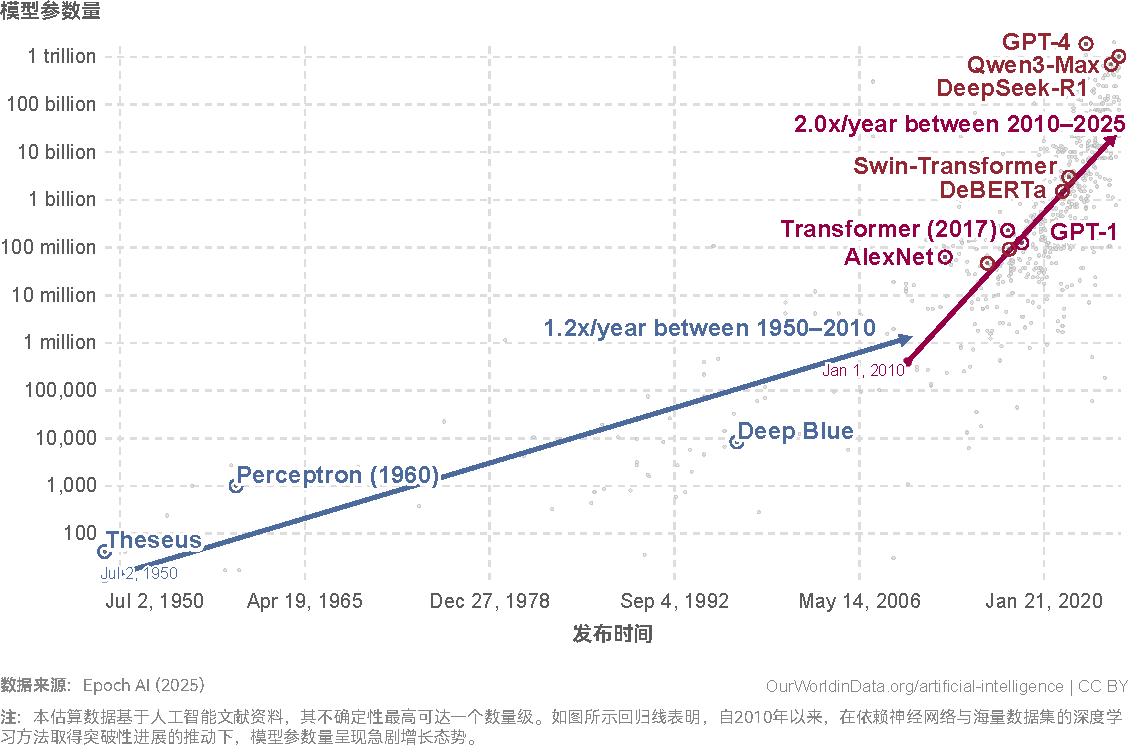
\includegraphics[width=.85\textwidth]{Ch1-1_model_parameter_evolve.pdf}
	\bicaption[典型人工智能系统参数规模的指数级增长趋势]{典型人工智能系统参数规模的指数级增长趋势。}[Exponential growth of parameters in notable AI systems]{Exponential growth of parameters in notable AI systems.}
	\label{fig:Ch1-1_model_parameter_evolve}
\end{figure}

然而,深度学习模型性能的飞跃,是以计算资源和能耗的大幅增加为代价的。模型规模、架构复杂度和计算量的膨胀几乎与性能提升同步发生。以上述 GPT-3 为例,其卓越的语言能力背后是极其高昂的参数优化成本(即训练开销)\cite{languagemodelsare_brown_2020}。公开资料与测算显示,大型模型训练消耗巨量算力并带来显著碳排放\cite{energypolicyconsiderations_strubell_2019,carbonfootprintmachine_patterson_2021}。更先进的 GPT-4,其训练投入的算力与成本更是远超于此\cite{gpt4technical_openai_2023}。这种“烧算力、堆数据”的模式引发了学术界和工业界对可持续性的广泛担忧,催生了“绿色 AI”的理念,倡导在追求性能的同时注重能效比\cite{energypolicyconsiderations_strubell_2019}.

更严峻的是,即使经过昂贵的训练,高性能模型的应用部署亦面临重重困难。庞大的模型在推理阶段同样需要海量算力支撑:一方面,动辄上万亿的参数规模需要数百 GB 内存空间;另一方面,惊人的浮点运算次数导致模型在资源受限环境中几乎无法运行,即便在云端也意味着巨大的运维成本和能耗。为此,业界与学界积极探索缓解上述矛盾的途径,例如:通过网络剪枝、权重量化等模型压缩技术削减参数规模\cite{deepcompressioncompressing_han_2016,quantizationtrainingneural_jacob_2018};通过知识蒸馏将大型模型的知识提炼到小模型中\cite{distillingknowledgeneural_hinton_2015};以及开发高效的专用 AI 加速器\cite{datacenterperformanceanalysis_jouppi_2017}。这些手段在一定程度上缓解了模型部署难题,但各有局限,尚无法从根本上扭转模型规模膨胀所带来的效率困境。

引发规模–效率矛盾的深层原因在于硬件发展和数据增长之间的不匹配。一方面,摩尔定律红利正在消退\cite{chipsaremoores_waldrop_2016}。近十年来,半导体工艺逼近物理极限,通用处理器性能提升速度显著放缓。尽管 GPU 和 TPU 等专用加速器提供了更高并行度,但硬件性能增长已无法线性支撑软件需求的激增。另一方面,大数据时代的来临使得可用于训练的数据量呈爆炸式增长。庞大的数据涌现为训练更大模型提供了燃料,也在客观上推动着模型朝更高复杂度、更深层数的架构发展。数据规模、架构复杂度和模型参数三者的同步扩张叠加,使得深度学习对计算资源的需求以史无前例的速度增长。当硬件算力的供给跟不上数据和模型的需求时,效率问题便不可避免地凸显出来。由此可见,摩尔定律放缓与数据爆炸这两股相反趋势共同作用,形成了性能提升与资源受限之间日益扩大的鸿沟。如何弥合这一鸿沟、化解规模与效率的矛盾,成为当前深度学习领域迫切需要解决的关键问题。

\mysubsection{深度模型构建的机理分析与关键环节}\label{sec:ch1-1-2-deep-model-mechanisms-and-key-steps}

要真正破解 \ref{sec:ch1-1-1-deep-learning-overview} 节所述的“规模-效率矛盾”,需要从深度模型构建的源头出发,辨析其核心组成与效率瓶颈。通过对大量成功模型的构建过程进行归纳与抽象,可以发现,深度模型的构建过程普遍包含三个相辅相成的关键环节:知识获取、结构承载和参数实现,如图~\ref{fig:three_stage_of_training} 所示。该划分并非严格的层级框架,而是为理解模型构建的复杂性提供了三个核心分析维度,也对应了前文所述三类成本的来源。

\begin{figure}
	\centering
	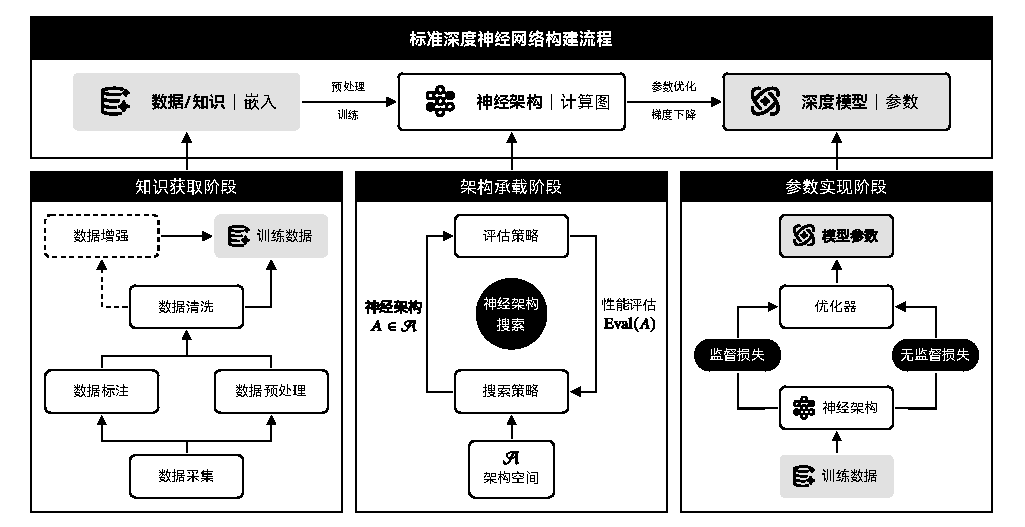
\includegraphics[width=\textwidth]{Ch1-1_three_stage_of_training.pdf}
	\bicaption[深度模型构建的三阶段机理框架]{标准深度模型构建的三阶段机理框架。}[Three-stage framework for deep model construction]{Three-stage framework for deep model construction.}
	\label{fig:three_stage_of_training}
\end{figure}

\textbf{(1)知识获取环节。}
知识获取是模型构建的基础,旨在通过数据的采集、标注和预处理来获取任务相关的先验知识。在这一环节,研究者需要准备海量的领域相关数据(如图像、文本等),并进行清洗和标注,为模型学习提供清晰的指导信号。例如在图像分类任务中,ImageNet 这类大型数据集为模型提供了丰富的知识基础\cite{imagenetlargescale_deng_2009}。然而,获取海量高质量标注数据本身即代表了高昂的数据成本。高质量、大规模的训练数据是模型获取知识的源泉,直接决定了模型能够学到的模式和知识的上限。

\textbf{(2)结构承载环节。}
结构承载环节关注如何设计合适的神经网络架构来承载和表示所获取的知识。良好的结构设计应与任务知识特性相契合,以有效提炼信息。然而,架构设计本身即是一项复杂的成本:需要在模型表达能力与计算开销、训练难度之间进行权衡。例如,ResNet 架构通过残差单元解决了深层网络训练难题\cite{deepresiduallearning_he_2016};Transformer 架构通过自注意力机制捕获长程依赖\cite{attentionisall_vaswani_2017}。在实践中,结构设计或依赖人工经验,或借助自动化的神经架构搜索(Neural Architecture Search, NAS)技术\cite{neuralarchitecturesearch_elsken_2019,neuralarchitecturesearch_zoph_2017,dartsdifferentiablearchitecture_liu_2019},但后者往往引入较高的搜索开销。

\textbf{(3)参数实现环节。}
参数实现环节的目标是通过模型训练和优化,将抽象的网络结构转化为解决实际任务的具体模型。利用前两环节准备的数据与架构,采用反向传播等优化算法调整可训练参数\cite{learningrepresentationsback_rumelhart_1986},使模型对训练数据的预测误差逐步减小。当前主流的预训练-微调范式\cite{bertpretraining_devlin_2019},其预训练阶段本身即是极其耗时的参数实现过程,而微调则是参数针对下游任务的再优化。

综上所述,知识获取、结构承载与参数实现构成了深度模型构建的三个核心维度。它们共同决定了模型的最终性能和构建效率。1.1.1 节所揭示的“规模-效率矛盾”,其根源便在于这三个维度上日益增长的资源消耗。因此,寻求模型的高效构建,本质上即是在这三个维度上分别探寻提升效率的有效路径。本文后续研究将以此划分为基础,探讨如何分别在知识、结构和参数层面,引入迁移优化的思想,以缓解各自的效率瓶颈。

\mysubsection{本文研究命题与目标}
\label{sec:ch1-1-3-research-problem-and-goals}

前两节系统地分析了深度学习领域的规模-效率矛盾 ,并将其解构为知识获取(数据成本) 、结构承载(架构设计成本) 与参数实现(训练与优化成本)  三个关键环节的效率瓶颈。面对这些挑战,若仍沿袭从零开始的构建范式——即为每个新任务收集海量新数据、设计全新架构、从头训练所有参数——无疑将使资源消耗的困境愈发严峻。

然而,一个核心的观察是:在过往的模型构建过程中,大量的知识已经被固化在不同的载体中——无论是海量数据集中蕴含的模式、优秀架构中体现的设计经验,还是已训练模型中沉淀的参数权重。因此,一个更高效的构建范式应当是最大化地复用、调整 与迁移 这些已有的知识,而非一味地重复造轮。
这种复用先验知识的理念,正是知识迁移或广义上的迁移优化思想的精髓\cite{surveytransferlearning_pan_2010}。它为应对上述三类成本瓶颈提供了一条统一的哲学路径:

\begin{itemize}[leftmargin=3em]
	\item 面对数据成本,我们可以迁移已在大数据上训练好的模型知识,以辅助小样本任务的学习(如知识蒸馏)\cite{distillingknowledgeneural_hinton_2015}。
	\item 面对架构成本,我们可以迁移已在源任务上验证的优秀架构经验,以加速新任务的架构搜索(如可迁移 NAS 思路)\cite{learningtransferablearchitectures_zoph_2018,neuralarchitecturesearch_elsken_2019}。
	\item 面对参数成本,我们可以迁移多个已训练模型的参数,将其直接融合以实现能力的即时集成,从而规避高昂的(再)训练开销(如 Model Soup~\cite{modelsoupsaveraging_wortsman_2022} 与 Task Arithmetic~\cite{editingmodelstask_ilharco_2023})。
\end{itemize}

基于此,本文提出将“基于知识迁移的深度模型高效构建”作为核心研究命题。本文的研究路径并非构建一个包罗万象的多层次统一框架,而是将在 \ref{sec:ch1-1-2-deep-model-mechanisms-and-key-steps} 节所划分的三个关键环节上,分别独立地展开研究,探讨迁移优化思想在各个维度上的具体应用与实现。

% 在知识层迁移优化方面,本文旨在缓解知识获取环节对海量标注数据的高度依赖。在数据匮乏(如少样本)场景下,模型性能严重受限 。此时,将一个在海量数据上训练的、知识丰富的教师模型所蕴含的知识迁移至一个轻量的学生模型,即知识蒸馏 ,成为一种极具潜力的解决方案。然而,传统蒸馏方法自身也高度依赖数据,在标注稀缺时其迁移过程往往变得极不稳定 。因此,本研究的目标是:针对少样本分类任务,研究高效且稳定的知识迁移机制,探索如何融合多源教师信号(如提示学习 与对比学习 ),以实现低资源条件下的鲁棒知识蒸馏 。

% 在结构层迁移优化方面,本文聚焦于解决结构承载环节的效率瓶颈。NAS 虽能自动化设计高性能架构,但其高昂的搜索成本 和“搜索空间碎片化” 难题,导致设计经验难以复用。为此,可迁移 NAS(Transferable NAS, TNAS)应运而生,其核心思想是将在源任务上获得的架构知识迁移至目标任务。然而,现有 TNAS 方法大多局限于同构搜索空间 ,对于架构范式(如 CNN 与 Transformer)截然不同的异构任务 ,知识迁移仍是巨大挑战 。因此,本研究的目标是:研究跨异构搜索空间的架构经验复用方法,通过构建统一的架构表征与跨域映射机制,实现架构设计经验的高效迁移,以显著降低 NAS 的搜索开销 。

% 在参数层迁移优化方面,本文致力于应对参数实现环节高昂的训练开销。随着预训练模型的规模达到万亿级别 ,(再)训练的成本已变得难以承受 。与此同时,如何将多个不同专长(如数学、代码、语言)的已训练模型的能力集成为一个统一模型,是业界的迫切需求 。模型融合 作为一种免训练的参数迁移范式备受关注,但简单的参数平均等策略极易引发参数冲突和性能退化 。因此,本研究的目标是:研究免训练条件下的模型参数高效融合机制,探索如何通过知识图谱引导的多形式优化策略,在不进行额外梯度下降的前提下,高效、稳定地将多个预训练模型的参数进行迁移与融合,实现能力的即时集成 。

在知识层迁移优化方面,本文旨在缓解知识获取环节对海量标注数据的高度依赖。在数据匮乏(如少样本)场景下,模型性能严重受限。此时,将一个在海量数据上训练的、知识丰富的教师模型所蕴含的知识迁移至一个轻量的学生模型,即知识蒸馏,成为一种极具潜力的解决方案\cite{distillingknowledgeneural_hinton_2015}。然而,传统蒸馏方法自身也高度依赖数据,在标注稀缺时其迁移过程往往变得极不稳定。本文将探索少样本场景下高效且稳定的知识迁移机制,探索如何融合多源教师信号(如提示学习\cite{exploitingclozequestions_schick_2021,ptuningv2_liu_2021}与对比学习\cite{representationlearningcontrastive_oord_2018}),以实现低资源条件下的鲁棒知识蒸馏。

在结构层迁移优化方面,本文聚焦于解决结构承载环节的效率瓶颈。NAS 虽能自动化设计高性能架构,但却也面临高昂的搜索成本和“搜索空间碎片化”难题,导致设计经验难以复用\cite{neuralarchitecturesearch_elsken_2019,nasbench101_ying_2019}。现有 TNAS 方法大多局限于同构搜索空间\cite{emtnastransferring_liao_2023,evolutionarymultitaskconvolutional_zhou_2024},对于架构空间不同的异构任务,知识迁移仍是巨大挑战。因此,本研究将探讨跨异构搜索空间的架构经验复用方法,通过构建统一的架构表征与跨域映射机制,实现架构设计经验的高效迁移\cite{oncealltrain_cai_2020}。

在参数层迁移优化方面,本文致力于应对参数实现环节高昂的训练开销。随着预训练模型的规模达到万亿级别,(再)训练的成本已变得难以承受。与此同时,如何将多个不同专长(如数学、代码、语言)的已训练模型的能力集成为一个统一模型,是业界的迫切需求。模型融合作为一种免训练的参数迁移范式备受关注,但简单的参数平均等策略极易引发参数冲突和性能退化\cite{modelsoupsaveraging_wortsman_2022,gitrebasin_ainsworth_2023,mergingmodelsfisher_matena_2022}。因此,本研究将探索知识引导的模型参数融合机制,探索如何通过知识图谱引导的多形式优化策略,高效、稳定地将多个预训练模型的参数进行迁移与融合,实现能力的即时集成。



这三个目标分别对应深度模型构建的一个关键环节,本文后续章节将围绕这三个目标,分别展开深入的算法设计与实验验证。

\mysection{国内外研究现状}\label{sec:ch1-2-global-research-status}

在 \ref{sec:ch1-1-research-background-and-significance} 节明确了本文的研究背景、核心命题与具体目标之后,本节旨在系统回顾与本文研究密切相关的国内外研究现状。深入理解现有技术的发展脉络、关键方法及其固有的局限性,是论证本文研究必要性与创新性的基础。

鉴于本文的研究聚焦于深度模型构建过程中的知识获取、结构承载与参数实现三个关键环节,并旨在分别应用迁移优化思想提升其效率,本节的文献综述也将围绕这三个维度展开。我们将分别考察在知识层面(如何高效利用和传递知识以减少数据依赖)、结构层面(如何自动化且高效地设计网络架构)以及参数层面(如何低成本地优化、调整或复用模型参数)的代表性研究进展。

在每个维度的综述中,我们将不仅介绍主流的技术路径与方法,更重要的是,批判性地分析其存在的瓶颈与局限,特别是与本文研究目标(如少样本场景、异构空间迁移、模型参数融合)相关的挑战。通过揭示现有方法的不足,我们将进一步明确本文所提出的研究问题(见 \ref{sec:ch1-4-core-questions-and-contributions} 节)的价值与紧迫性。本节的组织结构如下:\ref{sec:ch1-2-1-knowledge-transfer-status-limitations} 节探讨知识层迁移的研究现状与局限;\ref{sec:ch1-2-2-structural-transfer-status-limitations} 节聚焦结构层迁移;\ref{sec:ch1-2-3-parameter-transfer-status-limitations} 节则分析参数层迁移。最后,\ref{sec:ch1-2-4-summary-and-opportunities} 节将对各层面的研究现状以及研究机遇进行总结。

\mysubsection{知识层迁移研究现状与局限}
\label{sec:ch1-2-1-knowledge-transfer-status-limitations}

知识层面的迁移优化是应对深度模型构建中高昂数据成本的核心策略之一。其根本动机在于,深度学习模型在新领域或新任务中的性能常因数据分布差异而显著下降。为此,研究者致力于发展能够在不同数据分布间有效传递和复用知识的技术。早期工作主要集中于迁移学习与领域自适应(Domain Adaptation, DA),旨在利用已有(源域)数据的知识来提升在缺乏标注的目标域上的模型性能\cite{surveytransferlearning_pan_2010}.

领域自适应的主流技术路径大致可分为几类。其一是特征对齐方法,其核心思想是通过显式地最小化源域与目标域在模型特征空间中的分布差异来实现知识迁移。例如,一些研究采用最大均值差异(Maximum Mean Discrepancy, MMD)等统计距离度量作为损失函数,强制深度网络提取的源域和目标域特征在高层表征上趋于一致\cite{learningtransferablefeatures_long_2015}. 另一些工作则通过相关性对齐(Correlation Alignment, CORAL)等策略来匹配源、目标特征分布的二阶统计量,以减小域间特征偏移\cite{deepcoralcorrelation_sun_2016}. 龙明盛等人提出的深度适应网络(DAN)及其后续改进(如联合适应网络 JAN)均是基于 MMD 或其变种进行深度特征对齐的代表性工作\cite{learningtransferablefeatures_long_2015,deeptransferlearning_long_2017}。
其二是基于对抗训练的方法。受生成对抗网络思想启发,Ganin 等人提出了领域对抗神经网络(Domain-Adversarial Neural Network, DANN),在特征提取器后附加一个域判别器,通过引入梯度反转层在训练中对抗学习域不变表示\cite{domainadversarialtraining_ganin_2017}。后续研究如条件域对抗网络(CDAN)进一步提升了对抗适应的效果\cite{conditionaladversarialdomain_long_2018}。
此外,还有基于重构或伪标签的方法。例如,利用 CycleGAN 等图像翻译技术将源域图像风格迁移至目标域\cite{unpairedimageimage_zhu_2017};或利用目标域未标注数据的自监督信号(如旋转预测)进行预训练\cite{unsupervisedrepresentationlearning_gidaris_2018};或采用迭代式的自训练策略,利用模型自身对目标域样本的预测生成伪标签,并将其加入训练集进行优化\cite{pseudolabelsimple_lee_2013}。

尽管领域自适应技术显著提升了模型在目标域缺乏标注时的性能,但其应用仍面临局限:当源域与目标域差异过大时,特征对齐的效果可能受限;复杂的对抗训练策略常引入训练不稳定性;且大多数 DA 方法依赖于源域数据的可访问性,这在隐私或数据壁垒场景下难以满足\cite{surveytransferlearning_pan_2010,conditionaladversarialdomain_long_2018}。更重要的是,DA 主要解决的是跨数据分布的迁移,而对于模型结构或容量差异间的知识传递,则需要更直接的机制。

知识蒸馏(Knowledge Distillation, KD)正是为此而生的一种更通用的模型间知识迁移范式\cite{modelcompression_bucilua_2006,distillingknowledgeneural_hinton_2015}。KD 最早由 Bucilua 等人提出,并由 Hinton 等人在 2015 年系统阐述,其核心思想是由一个性能更优、结构更复杂的大型教师模型来指导一个参数量更少、结构更简单的学生模型进行训练。教师模型的作用不仅在于提供正确的硬标签,更关键的是其输出的概率分布(即 logits)蕴含了类别间的相似性关系,即所谓的软标签或暗知识。例如,教师模型可能认为一张猫的图片与狗的相似度远高于与汽车的相似度,这种细微的概率差异为学生提供了比单一硬标签(仅指示猫)更丰富的监督信号。学生模型通过优化一个复合损失函数——既要拟合真实标签,也要模仿教师的软标签(通常通过最小化 KL 散度或交叉熵)——从而不仅学会正确分类,更能继承教师对类别间关系的理解,提升泛化能力。教师输出的概率分布(软标签)蕴含类别间的相似性关系,可通过温度平滑的 Softmax 进行暴露\cite{distillingknowledgeneural_hinton_2015}。即便教师与学生架构相同(自蒸馏),KD 也常能提升学生的泛化性能\cite{bornagainneural_furlanello_2018}。

随着研究的深入,知识蒸馏的形式也日益丰富。除了经典的基于输出层 logits 的蒸馏,研究者进一步探索了中间层知识的传递:特征蒸馏让学生的隐藏层表示逼近教师对应层的特征表示\cite{fitnetshintsthin_romero_2015,variationalinformationdistillation_ahn_2019,knowledgetransfervia_heo_2019,payingmoreattention_zagoruyko_2017}。对于同构模型,可以直接对齐;对于异构模型,则需引入适配器模块(如 FitNets 的 Hints 层、变分信息蒸馏 VID、激活边界 AB 等)\cite{fitnetshintsthin_romero_2015}来桥接特征空间的差异。关系知识蒸馏关注样本间或层间的关系结构,如对齐注意力图或特征相似度矩阵\cite{relationalknowledgedistillation_park_2019},使学生学习教师的全局推理模式。多教师/互学蒸馏通过集成多个教师的知识,为学生提供更多样化的视角,从而提升性能与鲁棒性\cite{deepmutuallearning_zhang_2018}。知识蒸馏已在计算机视觉与自然语言处理中广泛应用,包括大型预训练模型(如 BERT)的压缩\cite{tinybertdistillingbert_jiao_2020,distilbertdistilledversion_sanh_2019},成为连接知识层与参数层、实现模型高效部署的关键技术。

然而,尽管知识蒸馏在实践中成效显著,但其在数据高效性与迁移稳定性方面仍面临严峻挑战,特别是在本文关注的少样本场景下。首先,KD 的效果高度依赖教师模型的质量\cite{distillingknowledgeneural_hinton_2015,knowledgedistillationsurvey_gou_2021}。在少样本条件下,教师模型本身就是用极少量数据训练或微调得到的,其自身的知识可能存在偏差、过拟合甚至错误。学生模型在模仿这样的教师时,难免会继承甚至放大这些缺陷。其次,数据稀缺性严重制约了蒸馏过程的稳定性。经典的 KD 主要依赖教师的显性输出(logits 或软标签)。当可用于蒸馏的标注样本非常有限时(例如每类仅有十几个样本),学生模型极易过拟合教师在这些特定样本上的行为模式,而未能学习到其背后通用的判别知识。这种过拟合会导致学生模型在未见样本上的泛化能力急剧下降,甚至出现负迁移现象,即蒸馏后的性能反而不如直接用少量样本训练的学生模型。再者,少样本场景下,教师模型的输出分布可能过于自信,趋近于独热向量。这意味着其提供的暗知识非常有限,软标签与硬标签差异不大,蒸馏所能带来的额外信息收益大大降低。此外,传统蒸馏方法往往忽视了教师模型内部丰富的隐性知识,例如中间层特征所蕴含的语义信息和结构关系。在标注数据充足时,仅依赖输出层知识或许尚可;但在数据极度稀缺时,这些能够反映教师解题过程的隐性知识变得尤为宝贵。然而,如何有效地提取并迁移这些隐性知识,特别是当师生模型架构异构、容量差异悬殊时,特征对齐本身就非常困难,强行匹配可能适得其反。
与此同时,大规模预训练语言模型(Pre-trained Language Model,PLM)的崛起\cite{bertpretraining_devlin_2019,robertarobustlyoptimized_liu_2019,makingpretrained_gao_2021}与提示学习\cite{exploitingclozequestions_schick_2021,ptuningv2_liu_2021}的成功,为少样本学习带来了新的范式,但也给知识蒸馏带来了新的挑战。提示学习通过设计任务相关的提示模板,将下游任务(如文本分类)转化为 PLM 在预训练阶段所熟悉的格式(如掩码填充),从而能够有效激活 PLM 内部存储的知识,在仅需极少(甚至无需)标注样本的情况下取得优异性能。例如,PET\cite{exploitingclozequestions_schick_2021}、P-Tuning\cite{ptuningv2_liu_2021}等方法已证明提示学习在 Few-Shot 场景下的巨大潜力。我们因此拥有了性能强大的大型提示教师模型。然而,这些动辄数十亿甚至上万亿参数的大模型,其高昂的推理成本和存储开销严重制约了它们的实际部署。这就迫切需要将大型提示教师的知识蒸馏到轻量级的学生模型中。但提示学习也给知识蒸馏带来独特困难\cite{prefixtuningoptimizing_li_2021,powerscaleparameter_lester_2021,exploitingclozequestions_schick_2021,ptuningv2_liu_2021}:(1) 提示教师的输出空间通常是整个词汇表(预测 Mask 位置的词),而非固定类别数的 logits,这与传统 KD 的假设不同;(2) 提示学习所处的正是极度数据匮乏的环境,这使得前述少样本 KD 的所有挑战(教师过拟合、学生过拟合、暗知识不足、隐性知识难迁移)都更加尖锐。

综上所述,尽管知识迁移技术,特别是知识蒸馏,为模型压缩和性能提升提供了有力武器,但在低资源和少样本条件下,实现高效且稳定的知识传递仍然是一个悬而未决的关键瓶颈 。特别是在提示学习日益普及的背景下,如何克服数据稀缺性带来的挑战,将大型提示教师的知识鲁棒地迁移给小型学生模型,已成为亟待解决的前沿问题。这正是本文研究目标一(见 \ref{sec:ch1-1-3-research-problem-and-goals} 节)的核心切入点:亟需探索新的知识蒸馏机制,例如通过融合对比学习增强隐性知识迁移、利用多源教师信号(如未标注数据和预训练知识)弥补数据不足等手段,以解决少样本场景下的蒸馏退化问题,实现低资源条件下的高效模型构建。

\mysubsection{结构层迁移研究现状与局限}
\label{sec:ch1-2-2-structural-transfer-status-limitations}

结构层面的优化旨在解决深度模型构建过程中结构承载环节的效率瓶颈,即高昂的架构设计成本。深度神经网络的性能在很大程度上取决于其架构设计。回顾深度学习的发展史,模型架构经历了从早期相对简单的多层感知机,到引入卷积神经网络,再到解决深度训练难题的残差网络,以及在序列建模领域取得突破的循环神经网络及其变种(LSTM, GRU),最终到近年来在自然语言处理乃至计算机视觉领域占据主导地位的 Transformer 模型 。这些标志性的架构大多依赖领域专家的深厚经验、敏锐直觉以及大量的试错实验才得以诞生 。这种人工设计范式虽然产出了众多经典模型,但其固有局限性日益凸显:不仅时间与人力成本高昂,而且面对指数级增长的潜在结构组合,人工探索的范围极其有限,可能错过更优的架构 。此外,随着深度学习应用场景的多样化,为特定任务、特定数据集乃至特定硬件平台(如移动端)定制最优架构的需求激增,仅靠人工调整难以高效满足 。

为克服人工设计的局限性,NAS 应运而生,旨在通过自动化方法在预定义的搜索空间内寻找性能最优的网络结构\cite{neuralarchitecturesearch_zoph_2017,neuralarchitecturesearch_elsken_2019}。NAS 通常被形式化为一个双层优化问题:外层循环负责搜索或生成候选架构,内层循环则负责为每个候选架构训练权重并评估其性能 。根据外层搜索策略的不同,主流 NAS 方法展现出多样化的技术路径。一种重要的范式是基于强化学习的 NAS\cite{neuralarchitecturesearch_zoph_2017,learningtransferablearchitectures_zoph_2018}。该方法将架构生成视为序列决策过程,使用控制器(如 RNN)生成架构描述符,并根据架构评估性能(奖励信号)来优化控制器策略 。Zoph 和 Le 的开创性工作\cite{neuralarchitecturesearch_zoph_2017}及其后续改进 NASNet 证明了 RL 方法能够发现超越人类设计的架构,但其极高的采样效率低下导致计算成本极其高昂 。另一种主流策略是基于进化算法的 NAS\cite{regularizedevolutionimage_real_2019,efficienttwostage_hou_2021,cellbasedfast_dong_2023}。此方法将架构视为种群中的个体,通过模拟自然选择、交叉和变异等操作进行迭代优化 。例如,Real 等人提出的 AmoebaNet\cite{regularizedevolutionimage_real_2019}使用锦标赛选择和老化机制来进化高性能架构。EA 方法具有良好的全局探索能力和并行性,但早期同样面临评估次数多、收敛慢的问题\cite{surveyevolutionaryneural_liu_2020}。随后,基于梯度优化的 NAS(即可微分 NAS)带来了显著的效率提升\cite{dartsdifferentiablearchitecture_liu_2019,pcdartspartial_xu_2020}。通过引入连续松弛,该方法将离散的架构选择转化为可微的优化问题 。DARTS\cite{dartsdifferentiablearchitecture_liu_2019}是其中的代表,它为每个候选操作分配可学习的权重,通过梯度下降同时优化网络权重和架构权重,极大地降低了搜索成本。然而,可微分 NAS 也存在优化不稳定、易陷入局部最优等问题\cite{neuralarchitecturesearch_elsken_2019}。此外,基于代理模型或性能预测器的 NAS 策略也备受关注\cite{renasrelativisticevaluation_xu_2021,peepholepredictingnetwork_deng_2017}。这类方法通过训练一个轻量级模型来预测候选架构的性能,从而避免对每个架构进行昂贵的完整训练和评估 。例如,利用高斯过程、贝斯优化 或图神经网络\cite{practicalbayesianoptimization_snoek_2012,bananasbayesianoptimization_white_2021,archgraphacyclic_huang_2022}来建模架构与性能的关系,并指导采样过程。这些方法显著减少了评估次数,但预测精度和对初始数据的依赖是其关键挑战。值得一提的是,权重共享策略\cite{efficientneuralarchitecture_pham_2018,singlepathone_guo_2020}的提出,通过让搜索空间中的架构共享权重,使得评估架构性能时无需从头训练,也极大地提升了 NAS 的效率。

尽管上述方法在降低 NAS 的计算开销方面取得了显著进展,但传统 NAS 范式仍存在一个核心瓶颈:架构知识的复用不足\cite{neuralarchitecturetransfer_lu_2021}。大多数 NAS 算法都是针对单一任务、单一数据集进行优化的 。每当面对一个新的任务或场景时,往往需要从零开始重新执行整个搜索过程,即使新旧任务之间可能存在很高的相似性 。这种缺乏跨任务经验迁移的做法,不仅造成了大量的冗余计算和资源浪费,也使得先前任务中发现的优秀架构模式未能得到有效复用,极大地制约了 NAS 在实际应用中的效率和可扩展性 。其深层原因在于搜索空间的碎片化:不同任务、甚至不同 NAS 算法所采用的搜索空间定义差异巨大\cite{neuralarchitecturesearch_elsken_2019},缺乏统一的架构表示和比较基准\cite{nasbench101_ying_2019,natsbenchbenchmarking_dong_2022},使得架构知识难以跨越这些壁垒进行传递 。

为了解决这一问题,可迁移 NAS(Transferable NAS, TNAS) 的研究应运而生 。TNAS 的核心思想是在新(目标)任务的架构搜索中,借鉴或迁移先前(源)任务中学到的架构知识或搜索经验,从而加速收敛、减少搜索成本 。早期的实践\cite{learningtransferablearchitectures_zoph_2018,progressiveneuralarchitecture_liu_2018}表明,将在小数据集(如 CIFAR-10)上搜索到的优秀架构单元直接迁移到大数据集(如 ImageNet)上堆叠,可以取得极具竞争力的性能,验证了架构知识在一定程度上的可迁移性。后续研究进一步探索了更系统的迁移策略。例如,神经架构迁移 提出将源任务的最优架构作为目标任务搜索的起点进行微调。进化式 TNAS 则利用进化算法的群体智能和适应性,在迁移过程中对源架构进行调整和优化,以更好地适应目标任务。代表性工作如 EMT-NAS~\cite{emtnastransferring_liao_2023} 通过在多个相关任务间并行进化并交换优秀个体,实现架构知识的共享;MTNAS~\cite{evolutionarymultitaskconvolutional_zhou_2024} 则采用多任务遗传算法框架,协同优化多个任务的架构。这些方法在相关任务之间进行迁移时,确实能够显著节省总搜索时间并提升性能。此外,也有工作尝试训练跨任务的性能预测器,例如 CDP(Cross-Domain Predictor)~\cite{bridgegaparchitecture_liu_2022},利用源任务的数据来辅助目标任务的架构评估 。

然而,当前 TNAS 研究的一个显著局限在于,它们几乎都假设源任务和目标任务共享相同或高度相似的架构搜索空间,即在同构搜索空间内进行迁移\cite{emtnastransferring_liao_2023,evolutionarymultitaskconvolutional_zhou_2024}。无论是 EMT-NAS 还是 MTNAS,其实验设置通常局限于同一类网络范式(如都是 CNN 架构)和相似的搜索空间定义(如都基于 Cell 结构)。这种假设极大地限制了 TNAS 的适用范围 。在现实世界中,不同任务往往需要截然不同的架构类型 。例如,图像分类可能最适合 CNN,而机器翻译则依赖 Transformer;即使同为视觉任务,小数据集上的最优架构与大数据集上的最优架构在深度、宽度和模块选择上也可能大相径庭 。

当源域和目标域的搜索空间在操作算子集、拓扑连接规则、单元/层级结构等方面存在本质差异时,即面临异构搜索空间的挑战 ,现有的 TNAS 方法便捉襟见肘。由于架构的语言(表示方式)不兼容,源空间的优秀架构无法直接翻译或应用于目标空间\cite{nasbench101_ying_2019,natsbenchbenchmarking_dong_2022,dartsdifferentiablearchitecture_liu_2019},架构知识的迁移路径被阻断。如何打破搜索空间的壁垒,在更加广泛、更加异质的任务间实现架构设计经验的复用,成为 NAS 领域一个重要且尚未被充分解决的前沿问题 。

跨异构搜索空间的架构迁移面临着一系列独特的挑战。首先,一个基础性的障碍在于统一架构表示的缺失\cite{neuralarchitecturesearch_elsken_2019}。如何设计一种通用的表示方法,能够对来自不同搜索空间(如 CNN Cell vs Transformer Block)的架构进行统一编码、比较和操作,是实现跨空间比较与迁移的前提。其次,弥合异构鸿沟需要有效建模跨域性能关联。源域的高性能架构在目标域的表现难以直接推断。因此,如何建立跨空间的可比性能度量或预测模型,以指导迁移选择,是一个关键难题(现有如 CDP 等尝试仍有局限)。最后,设计有效的迁移策略并规避负迁移风险至关重要。需要机制能在迁移过程中对架构进行调整,使其适应目标需求,而非生硬移植导致性能下降。进化算法在此方面展现出潜力,可以通过种群初始化和变异交叉操作,在保留源架构优点的同时引入适应性调整\cite{cmaevolutionstrategy_hansen_2016,regularizedevolutionimage_real_2019},这与进化迁移优化及序贯迁移优化\cite{evolutionarysequentialtransfer_xue_2022,solutiontransferevolutionary_xue_2023}的思想不谋而合。

综上所述,尽管 NAS 和 TNAS 技术取得了长足进步,但在跨越异构搜索空间进行架构知识迁移方面仍存在巨大的研究空白 。这正是本文研究目标二(见 \ref{sec:ch1-1-3-research-problem-and-goals} 节)的核心动机:亟需研究和开发新的方法论,特别是通过构建统一的架构表示学习机制和鲁棒的跨域迁移优化策略,以实现异构任务间的架构经验复用,从而显著提升 NAS 的效率、通用性和实用性。

\mysubsection{参数层迁移研究现状与局限}
\label{sec:ch1-2-3-parameter-transfer-status-limitations}

参数层面的迁移优化旨在应对深度模型构建过程中参数实现环节的高昂成本,特别是(再)训练开销。深度模型的训练本质上是参数学习的过程。随着预训练-微调范式成为主流,如何有效地利用和调整已有模型的参数以适应新任务,成为提升效率的关键。传统的全参数微调虽然直接有效,但当模型规模达到数十亿乃至万亿级别时,对每个下游任务都进行全参数微调的计算和存储成本变得难以承受。

为了降低微调开销,近年来参数高效微调(Parameter-Efficient Fine-Tuning,PEFT)方法应运而生 。PEFT 的核心思想是在微调过程中仅更新模型参数的一小部分,同时冻结绝大部分预训练参数。例如,Adapter Tuning 在 Transformer 层中插入可训练模块\cite{parameterefficienttransfer_houlsby_2019},LoRA 通过低秩分解近似参数更新\cite{loralowrank_hu_2022},而 Prefix Tuning 或 Prompt Tuning 则添加可训练的连续向量\cite{prefixtuningoptimizing_li_2021,powerscaleparameter_lester_2021}。这些方法显著减少了训练资源需求,使得大型预训练模型适配下游任务更为可行。然而,PEFT 本质上仍是一种需要数据和梯度优化的训练过程。

在追求极致效率的驱动下,研究者开始探索完全免训练的模型能力集成范式,即模型融合\cite{modelmergingllms_yang_2024}。模型融合旨在直接将多个已训练模型的参数进行合并,以期获得一个兼具各源模型能力的新模型,而无需任何额外的梯度更新。这种范式若能成功,将极大地降低模型能力组合的成本。早期的实践,如简单的权重平均,有时被称为模型汤\cite{modelsoupsaveraging_wortsman_2022},在特定条件下(如融合相似任务的检查点)确能提升性能。任务算术\cite{editingmodelstask_ilharco_2023}则尝试通过对模型参数增量进行向量运算来合成能力。

然而,看似简洁的模型融合在实践中面临着严峻的稳定性挑战,尤其是在尝试融合多个、来源异质或任务差异较大的模型时,其效果往往难以预测且极易失败。这种不稳定性源于一系列深层且相互交织的因素。一个核心障碍在于参数语义的错位\cite{gitrebasin_ainsworth_2023}。由于神经网络内部存在排列对称性,不同模型独立训练后,即使架构相同,其内部单元的语义排列也可能迥异。直接合并这些位置对应但语义错位的参数,往往导致网络功能紊乱。尽管有研究提出通过参数重排列或寻找共享损失盆地来缓解此问题,但这些方法大多局限于特定条件。
进一步加剧融合难度的是深度网络固有的非线性特性,这常常导致非线性干涉与性能塌陷\cite{losssurfacesmode_garipov_2018,averagingweightsleads_izmailov_2018}。即使参数在语义上得以对齐,对两组(可能位于不同最优区域)参数进行线性组合,其结果也未必落在低损失区域。如果源模型的功能存在冲突,简单的权重组合很可能将融合参数置于损失函数的峭壁或高原上,导致性能骤降。模型内部各层复杂的非线性变换和层间依赖关系,也使得简单的逐层合并极易破坏这种平衡,最终导致输出失真。
此外,不同模型在优化状态与正则化策略上的差异也为稳定融合带来了障碍。各模型可能采用不同的优化器、学习率、正则化强度(如 L2 正则)乃至批归一化统计量。直接合并这些状态各异的参数可能导致信号尺度失衡、对输入分布的假设漂移,从而削弱融合模型在原任务上的表现,引发能力漂移。

更根本的问题在于,当前的模型融合实践往往缺乏坚实的理论指导来确定合并策略。在融合多个模型时,如何选择合并的顺序、确定各模型的权重比例,目前大多依赖启发式规则或经验性的尝试,使得整个过程带有很强的随机性和不确定性。这种炼金术般的操作方式严重制约了模型融合作为可靠工具的实用化。

为缓解上述挑战,研究者提出了一些改进策略,例如采用球面线性插值、参数裁剪与符号对齐(如 TIES-Merging~\cite{tiesmergingresolving_yadav_2023})或引入随机性(如 DARE~\cite{languagemodelsare_yu_2024})。近期也有工作尝试利用进化算法或贝叶斯优化来搜索更优的融合配置\cite{evolutionaryoptimizationmodel_akiba_2025}。这些方法在一定程度上提升了融合的成功率,但依然难以从根本上保证在融合大量异质模型时的稳定性和性能。现有方法大多将融合视为一个单阶段的优化问题,缺乏对模型间复杂关系的显式建模和利用。

综上所述,虽然参数层迁移技术正朝着更高效乃至免训练的方向发展,但在实现多个、特别是异质预训练模型能力的高效、稳定集成方面,仍存在显著的技术瓶颈。如何克服参数冲突、非线性干涉等难题,设计出鲁棒且可扩展的免训练模型融合框架,是当前大模型时代亟待解决的关键问题。这正是本文研究目标三(见 \ref{sec:ch1-1-3-research-problem-and-goals} 节)的研究动机:亟需探索新的模型参数融合范式,例如通过引入知识图谱显式建模模型间关系、采用多形式优化分解融合过程等策略,以实现免训练条件下的稳定、高效的多模型能力集成。

\mysubsection{小结与研究机遇}
\label{sec:ch1-2-4-summary-and-opportunities}

通过对深度模型构建过程中知识、结构与参数三个关键环节的国内外研究现状进行系统梳理与分析,我们可以清晰地看到,尽管各个层面均取得了显著进展,但在追求更高构建效率的目标下,各自仍面临着亟待突破的瓶颈。

在知识层面,虽然知识蒸馏等迁移技术为降低数据依赖提供了有效途径,但其在少样本场景下的稳定性和效率问题依然突出 。如何设计鲁棒的迁移机制,在标注数据极度稀缺时,依然能够高效、可靠地传递教师模型的知识,特别是对于提示学习这类新兴范式,仍是一个重要的研究机遇 。

在结构层面,NAS的自动化能力令人瞩目,但其高昂的计算成本和架构经验难以跨任务复用的问题,尤其是在面对异构搜索空间时的迁移失效,严重制约了其广泛应用 。开发能够打破搜索空间壁垒、实现通用架构知识迁移的新型 TNAS 方法,是提升自动化模型设计效率的关键所在。

在参数层面,免训练的模型融合范式展现出极致的效率潜力,然而在融合多个、特别是异质模型时所面临的参数冲突、性能退化和缺乏理论指导等稳定性挑战,使得这一极具吸引力的技术路径在实践中困难重重 。研究稳定、高效且可扩展的多模型参数融合机制,对于实现模型能力的即时按需组合具有重大价值。

综上所述,现有研究在知识获取效率(低资源)、结构设计效率(跨域复用)和参数集成效率(免训练稳定融合)三个维度上均存在明显的研究空白。这些空白不仅揭示了当前深度模型高效构建所面临的核心挑战,也直接催生并印证了本文在 1.1.3 节所提出的三个研究目标的必要性与前瞻性。正是为了应对这些挑战,本文将分别在知识、结构、参数三个层面展开针对性的研究,探索基于迁移优化思想的高效模型构建新方法。下一节将进一步凝练本文的研究动机与总体思路。

% \begin{sidewaystable}[htbp]
% 	\centering
% 	\caption{层面、代表方法及其核心思路、主要局限与研究机遇}\label{tab:methods_comparison}
% 	\begin{tabularx}{\linewidth}{cLLLL}
% 		\toprule
% 		\textbf{层面}   & \textbf{代表方法}                                                  & \textbf{核心思路}                               & \textbf{主要局限}                    & \textbf{研究机遇}                    \\
% 		\midrule
% 		\bfseries 知识层 & 领域自适应;\newline 知识蒸馏 ;\newline 提示学习 & 对齐数据分布;通过师生模型传递知识以压缩模型;利用提示激活预训练模型知识以适应下游任务 & DA 依赖源数据且稳定性不足;KD 在少样本场景下效率低且不稳定 & 研究少样本条件下的高效、稳定知识蒸馏机制,特别是面向提示学习模型 \\
% 		\bfseries 结构层 & 人工设计架构 ;\newline NAS ;\newline 可迁移 NAS         & 基于先验手工设计;通过算法自动化搜索最优结构;提升搜索效率               & 人工设计成本高;NAS 搜索开销巨大               & 研究跨异构搜索空间的架构知识迁移方法,构建统一架构表示与迁移机制 \\
% 		\bfseries 参数层 & 全参数微调;\newline 参数高效微调;\newline 模型融合                            & 调整部分或全部参数适应新任务;追求免训练的模型能力即时集成               & PEFT 仍需训练;模型融合面临严峻的稳定性挑战         & 研究稳定、高效且可扩展的免训练模型融合机制            \\
% 		\bottomrule
% 	\end{tabularx}
% \end{sidewaystable}

\mysection{研究动机与总体思路}\label{sec:ch1-3-research-motivation-and-overview}

承接前文对深度学习规模-效率矛盾的深入剖析(1.1 节)以及对现有模型构建方法在知识、结构、参数三个层面局限性的系统回顾(1.2 节),本节旨在系统性地阐述驱动本文研究的核心动机,并清晰地勾勒出据此形成的总体研究思路与论文布局。在明确了当前深度模型高效构建所面临的普遍性挑战与现有技术的不足之后,本节将聚焦于论证本文所采取的研究路径的合理性——即为何选择以知识迁移作为核心指导思想,以及如何将这一思想具体落实为本文的研究框架与内容安排。通过本节的阐述,旨在为读者理解本文后续章节的研究工作提供宏观的视角与逻辑指引。

\mysubsection{效率瓶颈驱动下的研究动机}
\label{sec:ch1-3-1-efficiency-bottleneck-motivation}

前文(1.1 节)已系统揭示了当前深度学习领域所面临的一个核心困境:一方面,模型性能的边界不断被推向新的高度,展现出解决复杂问题的强大潜力;但另一方面,这种进步越来越依赖于数据、算力与人力投入的指数级增长,形成了难以为继的规模-效率矛盾。无论是训练动辄万亿参数的巨型模型所需的天文数字般的计算资源与能耗 ,还是为特定任务收集和标注海量高质量数据的巨大成本 ,亦或是设计、验证新型网络架构所耗费的大量专家时间与实验迭代 ,都指向了一个共同的现实:传统的从零构建或暴力扩展模式正逼近其经济、环境乃至技术上的极限。性能提升的边际效益递减,而资源消耗的边际成本激增,这一趋势严重制约了深度学习技术的普惠化及其在资源受限场景下的应用落地 。

紧随其后,1.2 节的国内外研究现状分析进一步从模型构建的关键环节具体印证了这些效率瓶颈的普遍性与顽固性。在知识获取层面,尽管迁移学习与知识蒸馏等技术试图降低对标注数据的依赖,但在低资源(如少样本)场景下,知识传递的效率和稳定性仍面临严峻挑战,难以有效应对现实世界中普遍存在的数据稀缺问题 。在结构承载层面,NAS虽然实现了设计的自动化,但其高昂的搜索开销使得“为每个任务定制最优架构”的理想在实践中往往代价过高;更重要的是,现有架构经验难以在不同任务(特别是跨越异构搜索空间)之间有效复用,导致大量的重复探索与资源浪费 。在参数实现层面,即使是参数高效微调也无法完全消除训练成本,而追求极致效率的免训练模型融合范式,则因其固有的参数冲突与非线性干涉问题,在融合多个、特别是来源异质的模型时,其稳定性和最终性能往往难以保障 。

面对这些普遍存在于模型构建各个环节、阻碍效率提升的瓶颈,我们必须深刻反思现有的构建范式。一个核心的洞察是:在过往大量的模型研发实践中,宝贵的知识——无论是体现在大规模数据集中的复杂模式、凝结在成功架构中的设计原则,还是沉淀在已训练模型参数中的泛化能力——已经被大量地创造和积累下来。继续忽视这些既有知识,为每一个新问题都投入巨量资源进行重复的学习和探索,无疑是一种巨大的浪费。因此,一个更符合可持续发展理念、更具智慧的构建范式应当转向最大化地复用、迁移和适配这些先验知识。

这种“复用先验以提升效率”的理念,正是知识迁移或更广义的迁移优化这一研究思潮的核心精神。它并非特指某一种具体的技术,而是一种旨在通过利用过往解决相关问题所获得的知识或经验,来加速或改进当前问题求解过程的通用方法论思想。将这一思想应用于深度模型的高效构建,意味着我们试图在模型生命周期的各个阶段,系统性地寻找和利用可迁移的知识资产,以此作为应对前述三维效率挑战(数据、架构、参数)的统一哲学指引。通过设计精巧的迁移机制,在模型构建的各个环节——从数据处理到架构设计,再到参数初始化与调整——引入先验知识,有望显著降低对原始资源的依赖,从而在保证甚至提升模型性能的同时,大幅提高构建效率。

因此,本文的核心动机即在于此:由深度模型构建中普遍存在的效率瓶颈所驱动,我们旨在系统性地探索如何将迁移优化这一核心思想作为指导原则,分别应用于深度模型构建的知识、结构与参数三个关键环节,以针对性地应对各自面临的效率难题,最终为实现深度模型的高效、可持续构建提供新的理论视角与实践途径。

\mysubsection{本文研究思路与布局}
\label{sec:ch1-3-2-research-idea-and-structure}

基于 1.3.1 节确立的研究动机,即利用知识迁移思想应对深度模型构建中知识、结构与参数三个关键环节的效率瓶颈,本节将详细阐述本文据此设计的总体研究思路,并勾勒论文的整体布局与内容安排。

首先需要明确的是,本文的研究路径并非寻求构建一个包罗万象、试图统一所有环节的“多层次整体迁移框架”。深度模型的构建过程本质上是一个复杂的系统工程,其中知识的获取与表示(知识层)、架构的设计与承载(结构层)、参数的学习与实现(参数层),各自遵循着不同的规律,面临着独特的挑战,也提供了差异化的优化契机。鉴于此,本文采取了一种更为聚焦且务实的研究思路:即,以知识迁移作为贯穿始终的核心指导思想,深入到深度模型构建的知识、结构、参数这三个相对独立的维度,分别展开针对性的、深入的研究。我们旨在探索并验证,知识迁移这一通用理念如何在不同环节的具体问题中得到有效应用,以缓解各自的效率瓶颈。

具体而言,这三项研究虽然在技术方法和应用场景上各自独立,但它们共享同一个哲学内核:都致力于通过不同形式的知识迁移与复用,来显著提升特定环节的模型构建效率,从而共同服务于“深度模型高效构建”这一总体研究命题。它们分别代表了将知识迁移思想应用于不同知识载体(语义知识、结构模式、参数表征)的实践探索。

因此,本文的总体研究布局也围绕这三个维度的独立探索自然展开:

在知识层面,核心挑战在于模型对大规模标注数据的依赖。当数据稀缺时,直接训练往往效果不佳。知识迁移在此处的应用体现为:将已在大规模数据上学习到的丰富语义知识或判别能力,从一个教师模型迁移至资源受限下训练的学生模型。本文将聚焦于少样本场景下的知识蒸馏这一具体问题,研究如何克服传统蒸馏方法在此条件下的不稳定性。具体工作(详见第二章)将提出一种面向少样本提示学习模型的双重对比知识蒸馏方法,通过设计新的迁移机制(融合多源教师知识与对比学习策略),实现数据匮乏条件下的鲁棒知识迁移,提升知识获取环节的效率。

在结构层面,主要瓶颈在于神经网络架构设计的高昂成本与经验复用的困难。尤其是当任务需求变化导致所需架构范式(如从 CNN 到 Transformer)也随之改变时,知识迁移面临巨大障碍。知识迁移在此处的应用体现为:将在先前任务中探索和验证过的有效架构设计模式或搜索经验,迁移至新的架构设计任务中,以加速搜索过程。本文将重点关注跨异构搜索空间的架构知识迁移这一前沿难题。具体工作(详见第三章)将提出一个基于统一架构表示学习与进化迁移的 BRIDGE 框架。该框架通过学习架构的通用表示并建立跨域映射,旨在实现异构搜索空间之间的架构设计知识的高效迁移,从而大幅降低NAS的开销,提升结构承载环节的效率。

在参数层面,效率挑战主要体现在高昂的(再)训练成本以及多模型能力集成的复杂性与不稳定性上。知识迁移在此处则以一种更为直接的形式体现:即直接迁移和组合已训练模型的参数,以期在免训练的条件下快速构建具备复合能力的新模型。本文将深入研究免训练模型融合中的核心挑战——参数冲突与性能退化问题。具体工作(详见第四章)将提出 KG-MFTO 框架,引入知识图谱来显式建模模型间的关系,并采用多形式优化策略指导融合过程。该框架旨在通过知识引导,实现多个大型语言模型参数在零训练条件下的高效、稳定融合,提升参数实现环节的效率。

这三项分别聚焦于知识、结构与参数层面的研究工作构成了本文的主体内容,将在后续章节进行详细的理论阐述、算法设计与实验验证。通过这样的研究布局,本文期望能为深度模型在三个关键维度上的高效构建,分别提供有价值的理论见解与实践方案,共同推进“基于知识迁移的深度模型高效构建”这一核心研究命题。

\mysection{核心研究问题与主要贡献}\label{sec:ch1-4-core-questions-and-contributions}

在明确了本文的研究动机(1.3.1 节)与总体研究思路(1.3.2 节)——即以知识迁移思想为指导,分别在知识、结构、参数三个维度上独立展开高效构建研究——之后,本节将进一步凝练驱动这些研究的核心科学问题,并系统概述本文为回答这些问题所做出的主要理论与方法贡献。清晰地界定研究问题是确保研究工作聚焦且深入的前提,而概括主要贡献则旨在为读者提供本文创新价值的总体图景。

\mysubsection{核心科学问题的提出}
\label{sec:ch1-4-1-core-scientific-question}

基于前文对深度学习发展现状、核心挑战(1.1 节)与现有研究局限(1.2 节)的深入剖析,本文的研究聚焦于深度模型高效构建中的三个关键维度。为了系统性地推进研究,并为后续章节的探索提供明确指引,我们将 1.1.3 节提出的三个研究目标进一步凝练为以下三个相互独立、分别对应知识、结构与参数层面的核心科学问题。这些问题不仅直接回应了当前领域面临的效率瓶颈,也代表了在各自方向上亟待突破的前沿挑战。

第一个核心科学问题关注知识层面的迁移效率与稳定性,特别是在数据稀缺条件下的挑战。正如 1.2.1 节所述,尽管知识蒸馏等技术为利用先验知识提供了途径,但在少样本场景下,其效果往往因教师偏差、学生过拟合以及隐性知识难以有效传递等因素而大打折扣 。这不仅仅是一个简单的应用问题,更触及了知识表示与迁移的根本机制:当监督信号极其微弱时,模型如何区分并吸收真正有价值的知识,而非噪声或偏差?因此,本研究提出:在缺乏大量标注数据的条件下,如何设计高效且稳定的知识迁移机制,特别是探索新型知识蒸馏策略(例如结合对比学习或利用无标签数据),以从根本上克服少样本场景下的性能退化问题,并确保知识传递的鲁棒性? 回答这一问题,不仅能显著降低模型构建对昂贵标注数据的依赖,也将深化我们对低资源学习环境下知识表示与泛化机理的理解。

第二个核心科学问题聚焦于结构层面的知识复用效率,特别是在架构范式存在差异时的障碍。1.2.2 节的分析表明,NAS虽能自动化设计,但其高昂成本和一次性搜索模式限制了效率,而现有的可迁移 NAS又大多局限于同构搜索空间,难以应对跨越不同架构范式(如 CNN 与 Transformer)的场景 。这引出了一个核心的科学挑战:是否存在一种通用的架构知识表示方法,能够超越具体的算子和拓扑细节,捕捉架构设计的本质规律?如果存在,如何基于这种表示实现跨越异构搜索空间的有效知识迁移?因此,本研究提出:在计算资源有限的情况下,如何建立统一的神经架构表示学习框架,并设计相应的跨域迁移策略,以实现跨越不同架构范式(即异构搜索空间)的结构知识有效迁移,从而显著提升NAS的效率与通用性? 解决这一问题,不仅能大幅降低自动化模型设计的成本,更有望揭示不同架构家族之间潜在的设计共性与演化联系。

第三个核心科学问题则着眼于参数层面的免训练集成,旨在解决多模型能力组合的稳定性难题。1.2.3 节指出,免训练的模型融合作为一种极具吸引力的能力集成方式,因参数语义错位、非线性干涉等固有难题,在融合多个、特别是来源异质的模型时,其稳定性和性能保持面临严峻挑战 。这触及了深度模型参数空间几何特性以及多模型知识兼容性的基础问题:不同模型学习到的知识如何在参数层面进行有效的、非破坏性的叠加?是否存在一种无需梯度优化的机制,能够智能地识别并缓解参数冲突,保留各模型的核心能力?因此,本研究提出:在免训练条件下,如何设计系统化的参数融合框架,特别是引入显式的知识建模与优化策略,以实现多个下游专长模型间参数的高效、稳定融合,确保在有效集成各模型能力的同时,最大限度地避免性能损失?攻克这一难题,不仅能为即时、低成本地构建具备复合能力的强大模型开辟新途径,也将促进我们对大型模型参数空间结构及其组合规律的认识。

这三个核心科学问题共同构成了本文研究的出发点和落脚点。它们分别从知识传递、结构设计和参数集成三个维度切入深度模型高效构建的核心挑战,不仅具有重要的实践价值,也蕴含着深入探索深度学习内在机理的理论意义。本文后续章节提出的创新性解决方案,正是围绕这三个核心问题展开的直接回应。图~\ref{fig:research_questions} 直观地展示了本文围绕深度模型构建的知识、结构与参数三个层面,提出的核心科学问题 (Q1, Q2, Q3) 及其相应的研究目标。

\begin{figure}
	\centering
	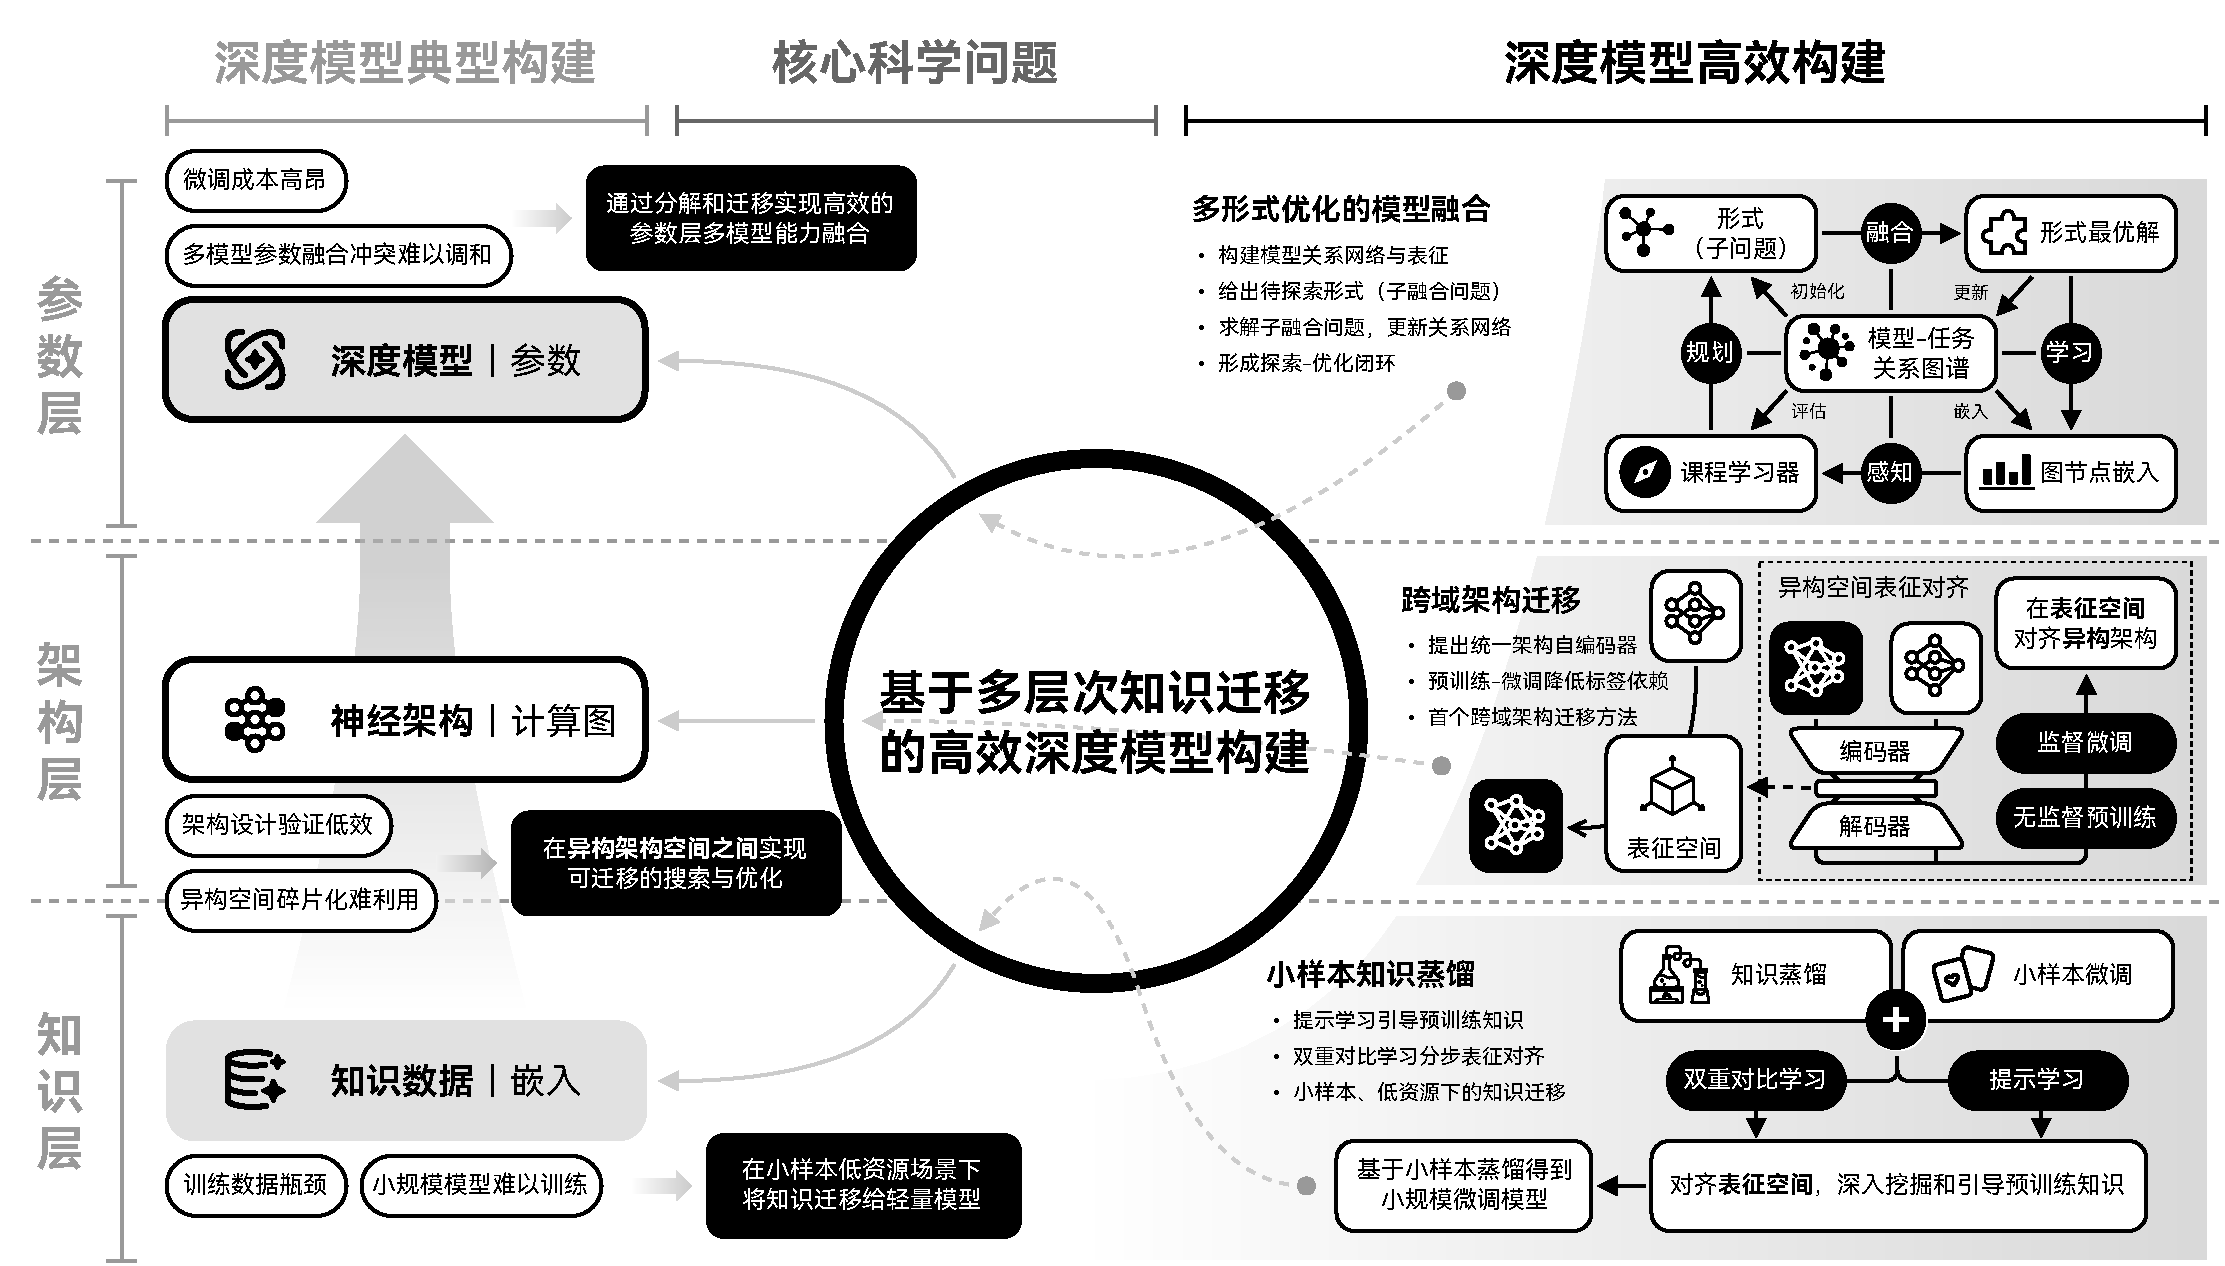
\includegraphics[width=\linewidth]{research_question.pdf}
	\bicaption[核心科学问题与研究目标]{本文围绕深度模型构建的知识、结构与参数三个层面,提出的核心科学问题及其相应的研究目标}[Core questions and objectives]{Core scientific questions and research objectives across the knowledge, structure, and parameter dimensions of deep model construction}\label{fig:research_questions}
\end{figure}

\mysubsection{主要贡献概述}
\label{sec:ch1-4-2-main-contributions-overview}

围绕 1.4.1 节提出的三个核心科学问题,本文分别在深度模型构建的知识、结构与参数三个层面展开了深入研究,并提出了一系列旨在提升构建效率的创新性方法。这些工作共同构成了本文对“基于知识迁移的深度模型高效构建”这一核心命题的具体探索与实践。本文的主要贡献可概括如下:

首先,针对知识层面在少样本条件下知识迁移效率与稳定性的核心问题 (Q1),本文提出了一种面向低标注场景的双教师对比蒸馏框架——Prompt-Distiller 。该方法创新性地融合了来自提示微调教师的任务特定知识(显性输出)与来自原始预训练教师的通用语言知识(通过无标注数据蒸馏),并通过引入一种基于探针的对比学习策略来增强对教师模型中间层隐性知识的迁移。与传统知识蒸馏方法在少样本数据下容易失效或不稳定的问题不同,Prompt-Distiller 通过多源、多层次的知识信号协同指导,显著提升了学生模型在数据匮乏环境下的性能与鲁棒性。实验证明(详见第二章),该方法能够有效克服少样本蒸馏的退化现象,为低资源场景下的模型压缩与高效构建提供了一种有效的知识迁移解决方案 。

其次,为应对结构层面跨异构搜索空间进行架构知识迁移的挑战 (Q2),本文构建了一个统一的神经架构表示学习与迁移框架——\textsc{Bridge} 。该框架的核心在于突破了现有可迁移 NAS 局限于同构搜索空间的限制。通过设计定制化的神经架构分词器与基于 Transformer 的变分自编码器,\textsc{Bridge} 能够将来自不同搜索空间(如基于 CNN Cell 和基于 Transformer Block)的架构映射到统一的、结构感知的潜在表示空间。在此基础上,我们进一步设计了跨域表示映射学习策略与进化序贯迁移优化 算法,能够将源任务中发现的优秀架构经验显式地迁移并适应到目标任务的异构搜索空间中。实验结果表明(详见第三章),\textsc{Bridge} 框架能够在显著降低 NAS 搜索成本(减少约 50\% 的 GPU 时长)的同时,发现与从零搜索相当甚至更优的高性能架构,为实现跨任务、跨架构范式的自动化模型设计经验复用提供了可行路径。

最后,针对参数层面免训练模型融合的稳定性难题 (Q3),本文提出了一种利用模型关系知识图谱指导的多形式优化范式——KG-MFTO 。该方法将复杂的多模型融合问题分解为一系列更易于求解的子问题(形式),并创新性地引入动态演化的知识图谱来显式建模和记录模型间的协同与冲突关系。通过课程规划器自适应地选择优化形式序列,并利用知识图谱引导的进化求解器(热启动 CMA-ES)高效搜索融合参数,KG-MFTO 能够在无需任何额外训练的条件下,稳定、高效地整合多个(特别是来源异质的)大型预训练模型的能力。实验验证(详见第四章),该方法在融合多个 LLM 专长模型时,能够有效缓解参数冲突,显著提升融合后模型在多任务上的综合性能与稳定性,优于现有的静态融合或无指导搜索方法,为实现模型能力的即时、低成本集成提供了一种全新的、基于知识迁移优化的解决方案 。

综上所述,本文通过在知识、结构、参数三个层面分别提出的 Prompt-Distiller、\textsc{Bridge} 和 KG-MFTO 方法,为深度模型的高效构建提供了具体的技术支撑。这些贡献不仅在各自领域内拓展了知识迁移的应用边界,也共同印证了以知识迁移思想应对模型构建效率瓶颈的有效性与潜力。

\mysection{论文结构安排}\label{sec:ch1-5-thesis-structure}

\begin{figure}[t]
	\centering
	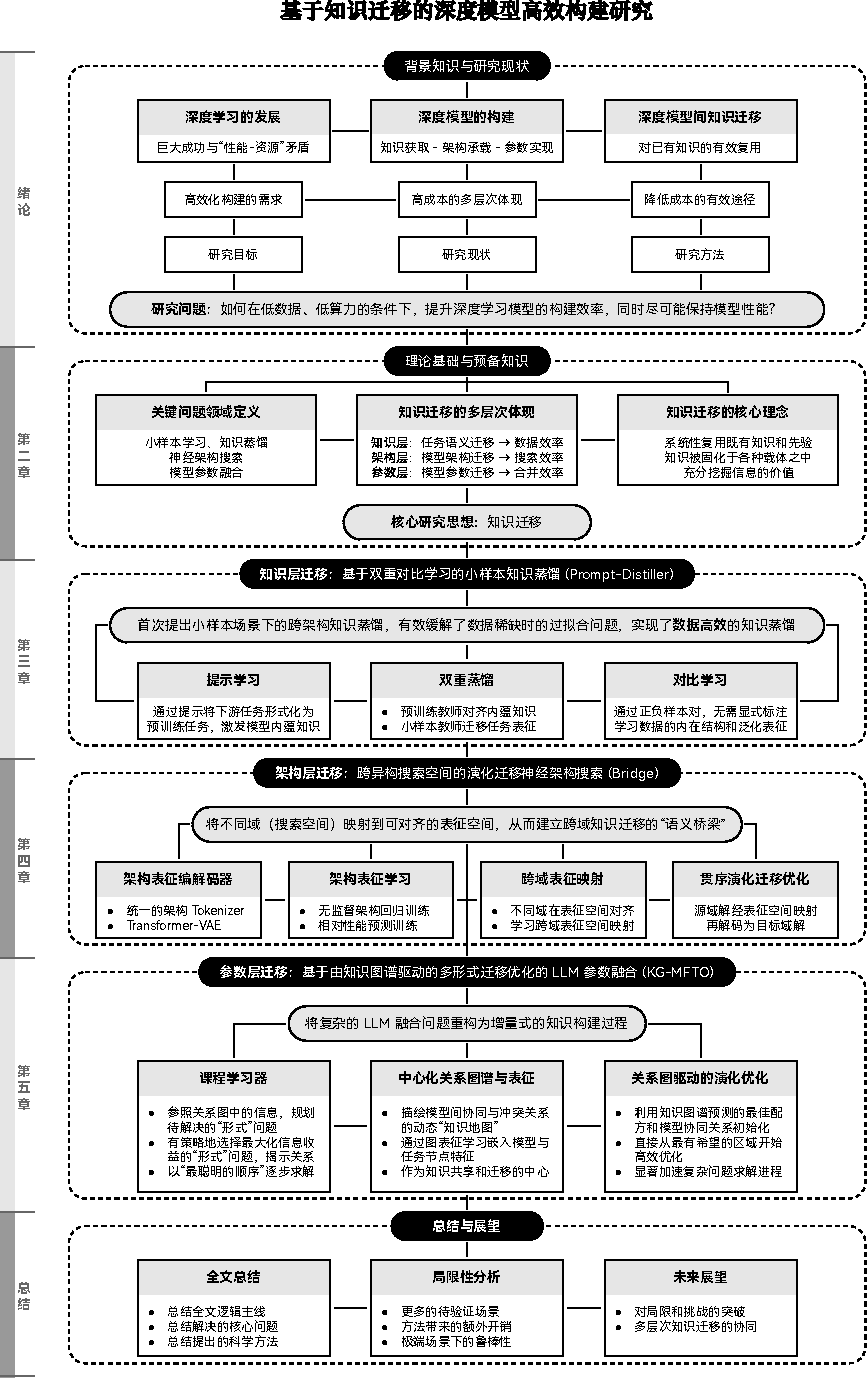
\includegraphics[width=.92\linewidth]{overall_struction-crop.pdf}
	\bicaption[论文结构示意图]{本文整体结构安排示意图}[Thesis structure]{Overall structure of this thesis}\label{fig:overall_structure}
\end{figure}

本文围绕“基于知识迁移的深度模型高效构建”这一核心命题,分别在知识、结构与参数三个维度展开研究。全文共分为五个主要章节,如图~\ref{fig:overall_structure}所示,其结构安排如下:

第一章:绪论。本章首先阐述了研究背景,指出了深度学习发展中日益严峻的规模-效率矛盾,并将其解构为知识获取、结构承载与参数实现三个关键环节的效率瓶颈。随后,提出了本文以知识迁移思想应对这些瓶颈的核心研究命题与三个具体研究目标。接着,通过回顾国内外相关研究现状,进一步明确了本文研究的切入点与创新性。最后,凝练了核心科学问题并概述了主要贡献,为全文奠定了研究基础和论述框架。

第三章聚焦于知识层迁移研究,详细阐述了面向少样本提示学习模型的双重对比知识蒸馏方法。该章节将深入探讨 Prompt-Distiller 的理论框架、算法设计(包括双教师机制与对比学习策略)及其实现细节,并通过大量实验验证其在低资源条件下提升知识迁移效率与稳定性的有效性。

第四章转向结构层迁移研究,提出了旨在解决跨异构搜索空间架构知识迁移难题的 BRIDGE 框架。本章将重点介绍其统一神经架构表示学习机制、跨域表示映射方法以及进化序贯迁移优化策略,并通过理论分析与实验评估,展示 BRIDGE 在实现高效、通用 NAS 方面的能力。

第五章则深入探讨参数层迁移研究,提出了面向大语言模型参数融合的知识引导多形式优化方法。该章节将详细介绍如何利用知识图谱、课程规划与知识引导的进化求解器,在零训练条件下实现多个 LLM 参数的高效、稳定融合,并验证其性能与效率优势。

第六章:总结与展望。本章将对全文的研究工作进行系统性总结,再次凝练本文在知识、结构、参数三个层面所提出的主要方法、核心贡献及其意义。同时,本章也将客观分析当前研究存在的局限性,并基于此对未来可能的研究方向(如多模态迁移、持续学习场景下的高效构建等)进行展望。

此外,附录部分提供了作者在攻读学位期间发表的论文目录、参与的科研项目以及本研究所使用的部分数据集信息。

\end{document}
